% Options for packages loaded elsewhere
\PassOptionsToPackage{unicode}{hyperref}
\PassOptionsToPackage{hyphens}{url}
\PassOptionsToPackage{dvipsnames,svgnames,x11names}{xcolor}
\documentclass[
  10pt,
]{ltjsarticle}
\usepackage{xcolor}
\usepackage[margin=16mm]{geometry}
\usepackage{amsmath,amssymb}
\setcounter{secnumdepth}{-\maxdimen} % remove section numbering
\usepackage{iftex}
\ifPDFTeX
  \usepackage[T1]{fontenc}
  \usepackage[utf8]{inputenc}
  \usepackage{textcomp} % provide euro and other symbols
\else % if luatex or xetex
  \usepackage{unicode-math} % this also loads fontspec
  \defaultfontfeatures{Scale=MatchLowercase}
  \defaultfontfeatures[\rmfamily]{Ligatures=TeX,Scale=1}
\fi
\usepackage{lmodern}
\ifPDFTeX\else
  % xetex/luatex font selection
\fi
% Use upquote if available, for straight quotes in verbatim environments
\IfFileExists{upquote.sty}{\usepackage{upquote}}{}
\IfFileExists{microtype.sty}{% use microtype if available
  \usepackage[]{microtype}
  \UseMicrotypeSet[protrusion]{basicmath} % disable protrusion for tt fonts
}{}
\makeatletter
\@ifundefined{KOMAClassName}{% if non-KOMA class
  \IfFileExists{parskip.sty}{%
    \usepackage{parskip}
  }{% else
    \setlength{\parindent}{0pt}
    \setlength{\parskip}{6pt plus 2pt minus 1pt}}
}{% if KOMA class
  \KOMAoptions{parskip=half}}
\makeatother
\usepackage{longtable,booktabs,array}
\newcounter{none} % for unnumbered tables
\usepackage{calc} % for calculating minipage widths
% Correct order of tables after \paragraph or \subparagraph
\usepackage{etoolbox}
\makeatletter
\patchcmd\longtable{\par}{\if@noskipsec\mbox{}\fi\par}{}{}
\makeatother
% Allow footnotes in longtable head/foot
\IfFileExists{footnotehyper.sty}{\usepackage{footnotehyper}}{\usepackage{footnote}}
\makesavenoteenv{longtable}
\usepackage{graphicx}
\makeatletter
\newsavebox\pandoc@box
\newcommand*\pandocbounded[1]{% scales image to fit in text height/width
  \sbox\pandoc@box{#1}%
  \Gscale@div\@tempa{\textheight}{\dimexpr\ht\pandoc@box+\dp\pandoc@box\relax}%
  \Gscale@div\@tempb{\linewidth}{\wd\pandoc@box}%
  \ifdim\@tempb\p@<\@tempa\p@\let\@tempa\@tempb\fi% select the smaller of both
  \ifdim\@tempa\p@<\p@\scalebox{\@tempa}{\usebox\pandoc@box}%
  \else\usebox{\pandoc@box}%
  \fi%
}
% Set default figure placement to htbp
\def\fps@figure{htbp}
\makeatother
\setlength{\emergencystretch}{3em} % prevent overfull lines
\providecommand{\tightlist}{%
  \setlength{\itemsep}{0pt}\setlength{\parskip}{0pt}}
\usepackage{bookmark}
\IfFileExists{xurl.sty}{\usepackage{xurl}}{} % add URL line breaks if available
\urlstyle{same}
\hypersetup{
  colorlinks=true,
  linkcolor={Maroon},
  filecolor={Maroon},
  citecolor={Blue},
  urlcolor={Blue},
  pdfcreator={LaTeX via pandoc}}

\author{}
\date{}

\begin{document}

\section{ハンズアウト:波長空間と周波数空間の双対幾何 ──
全16論文+総説(v2、2026-06-12
全篇公開)}\label{ux30cfux30f3ux30baux30a2ux30a6ux30c8ux6ce2ux9577ux7a7aux9593ux3068ux5468ux6ce2ux6570ux7a7aux9593ux306eux53ccux5bfeux5e7eux4f55-ux516816ux8ad6ux6587ux7dcfux8aacv22026-06-12-ux5168ux7bc7ux516cux958b}

\textbf{木原範昭(WF System Co., Ltd.~/ ORCID: 0009-0004-6753-4020)・CC
BY 4.0}

\subsection{一枚で言うと}\label{ux4e00ux679aux3067ux8a00ux3046ux3068}

仮定は三つ ---
\textbf{νλ=1(関係ひとつ)・零点½(定数ひとつ)・非対称1ビット} ---
に運用原理二つ(配置読み・記録原理)。この在庫だけから、量子的・時空的に見える構造がどこまで\textbf{定理として}従うかを、全段機械検算可能な離散系で確かめた観察シリーズ。全16論文+総説、日英バイリンガル、Zenodo
公開済み。\textbf{物理的同一視は行わない}(中心テーゼ:同じ結果の別写像)。

\subsection{シリーズ地図}\label{ux30b7ux30eaux30fcux30baux5730ux56f3}

{\def\LTcaptype{none} % do not increment counter
\begin{longtable}[]{@{}
  >{\raggedright\arraybackslash}p{(\linewidth - 4\tabcolsep) * \real{0.3333}}
  >{\raggedright\arraybackslash}p{(\linewidth - 4\tabcolsep) * \real{0.3333}}
  >{\raggedright\arraybackslash}p{(\linewidth - 4\tabcolsep) * \real{0.3333}}@{}}
\toprule\noalign{}
\begin{minipage}[b]{\linewidth}\raggedright
篇
\end{minipage} & \begin{minipage}[b]{\linewidth}\raggedright
論文
\end{minipage} & \begin{minipage}[b]{\linewidth}\raggedright
内容
\end{minipage} \\
\midrule\noalign{}
\endhead
\bottomrule\noalign{}
\endlastfoot
基礎 & 1〜4 & 格子と計数:\(N_0\)(R)=1, 9, 137,
\ldots(純粋な数え上げ)、分裂、階層真空 \\
定理 & 5〜12 &
辞書定理・凍結定理(時間の条件=1ビット)・排他の定理化・面積則・半波長検閲・創発ゲージ・\textbf{次元4の必然性}・測定=記録の追記 \\
続報 & 13〜16 &
\textbf{位置と時間の解決}・時間方向=複素構造・座標写像の構成検証・\textbf{測度問題の縮約} \\
総説 & --- & 標準理論への辞書と\textbf{公理の交換収支} \\
\end{longtable}
}

\subsection{続報編(2026-06-12
公開)の主結果}\label{ux7d9aux5831ux7de82026-06-12-ux516cux958bux306eux4e3bux7d50ux679c}

\textbf{論文13
位置は読まれていなかった}:離散位置=波の符号セクター(状態追加ゼロ)。空間=保存量格子の
Pontryagin 双対(三対称性は双対性の定理)。読み出し三層
\textbf{11⊂13⊂21}(強度縞は情報の約半分を原理的に失う)。時計標的=\textbf{全奇数
--- ガウスの三角数定理による証明付き}。t は導出量(独立逆写像なし)。

\textbf{論文14
時間方向と振幅の舞台}:時間方向の選択=複素構造の選択(格子互換な複素構造はちょうど16個、\(B_4\)
単一軌道)。輸送位相は導出され\textbf{例外なく \(Z_4\)}
に着地。対称化公準 → \textbf{正準規約定理}(集合構造の帰結)。

\textbf{論文15 xyztRQ への射影}:状態 → (x,y,z,t,R,Q)
の明示的写像・逆写像を5段の演算として構成、\textbf{往復500/500・保存則と可換}(電荷様パリティ=台の算術の定理:違反候補39.2\%に対し寄与経路の違反ゼロ)。速度は記録の列にのみ存在。

\textbf{論文16
測度問題の厳密な縮約}:集計規則は\textbf{選定しない}。歴史的近接0.0007=二結果圧縮の見かけ(3結果で乖離は3桁跳躍)。干渉粒度は規約でない:鏡像親が
\textbf{W=0(厳密)∧
W′=768(厳密)}。残る自由度を\textbf{粒度×イベント1ビット×条件付け}に縮約し、判定実験の表をモデル内部に設置。Born
則=「然るべき極限で合流すべき有効則」(収束・抑制・予言の三つ組基準)。

\begin{figure}
\centering
\pandocbounded{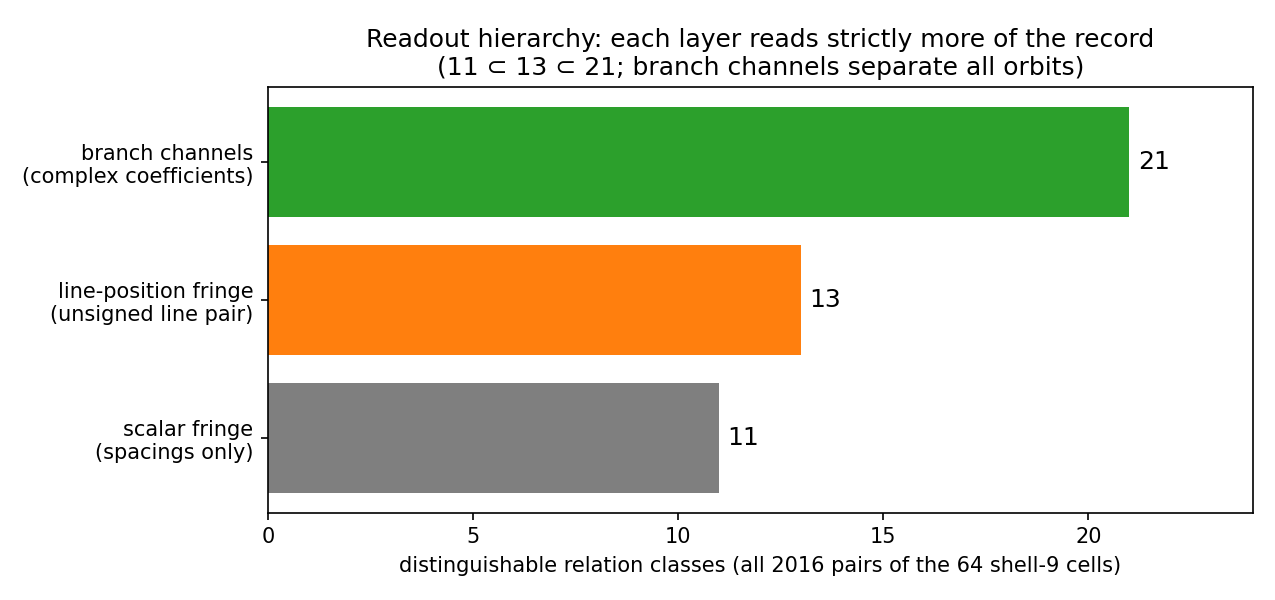
\includegraphics[keepaspectratio,alt={読み出し三層 11⊂13⊂21}]{paper13_fig2_readout_layers.png}}
\caption{読み出し三層 11⊂13⊂21}
\end{figure}

\begin{figure}
\centering
\pandocbounded{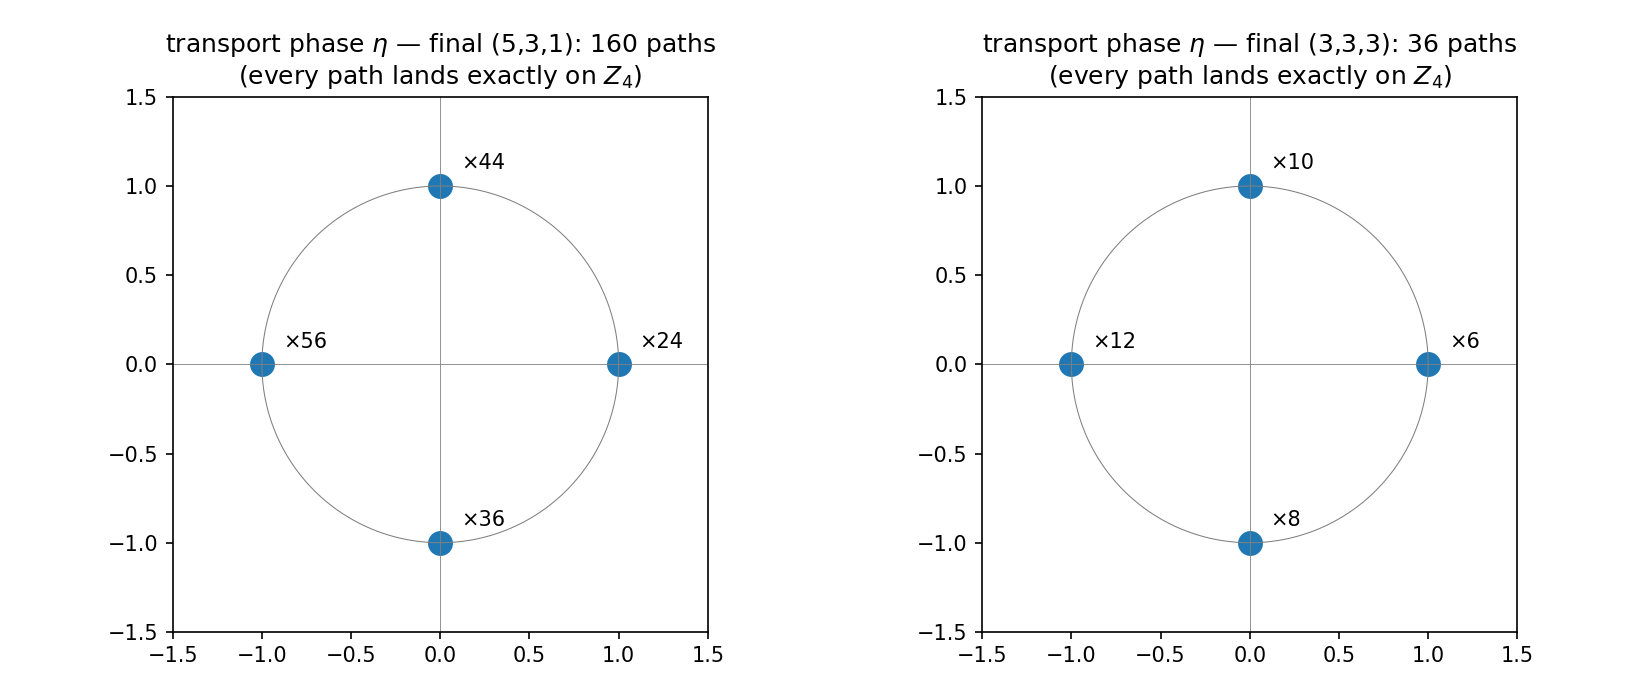
\includegraphics[keepaspectratio,alt={輸送位相は例外なく Z\_4 に着地}]{paper14_fig1_eta_z4.png}}
\caption{輸送位相は例外なく \(Z_4\) に着地}
\end{figure}

\begin{figure}
\centering
\pandocbounded{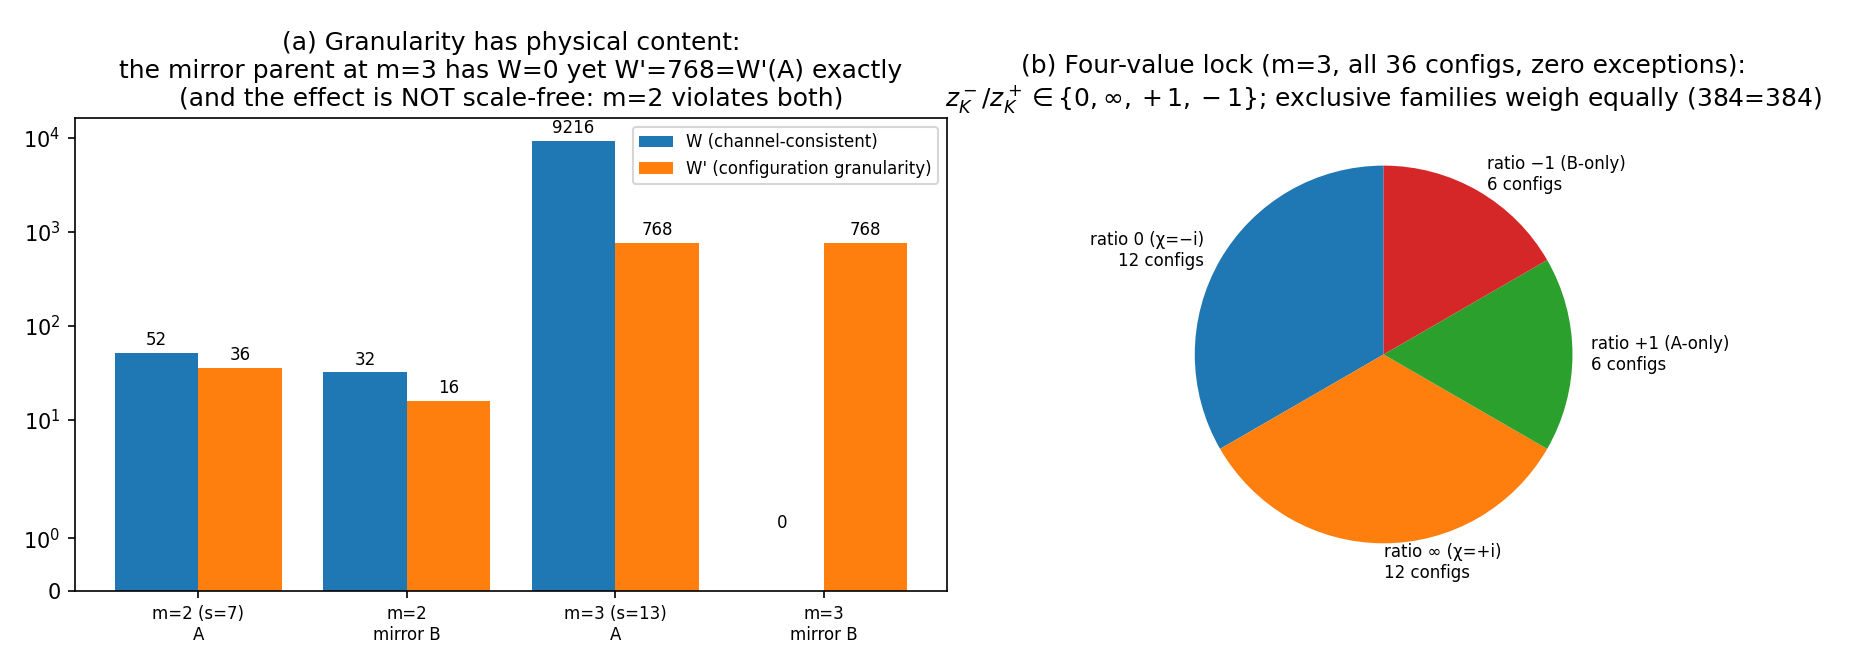
\includegraphics[keepaspectratio,alt={干渉粒度の非規約性と四値ロック}]{paper16_fig3_granularity.png}}
\caption{干渉粒度の非規約性と四値ロック}
\end{figure}

▲
上から:読み出し三層(強度縞11⊂線位置13⊂枝チャネル21=完全分離、論文13)/輸送位相の
\(Z_4\) 着地(全196経路・例外ゼロ、論文14)/鏡像相殺 W=0∧W′\textgreater0
と四値ロック(論文16)。全図実計算。

\subsection{総説:公理の交換収支}\label{ux7dcfux8aacux516cux7406ux306eux4ea4ux63dbux53ceux652f}

{\def\LTcaptype{none} % do not increment counter
\begin{longtable}[]{@{}lll@{}}
\toprule\noalign{}
標準理論では公理 & 本体系では & 出典 \\
\midrule\noalign{}
\endhead
\bottomrule\noalign{}
\endlastfoot
対称化公準 & \textbf{定理}(正準規約) & 論文14 \\
時間=外部パラメータ & \textbf{定理}(導出量) & 論文13・15 \\
測定公準 & \textbf{定理}(追記+記録) & 論文12 \\
時空次元=入力 & \textbf{定理}(必然性) & 論文11 \\
電荷保存 & \textbf{定理}(台のパリティ算術) & 論文15 \\
\end{longtable}
}

支払い:関係1+定数1+1ビット+運用原理2。\textbf{未記入は測度と作用の二項のみ}。テーゼ:完全に埋まった辞書=再記法=経験的内容ゼロ。\textbf{接続が不完全な点こそ、観測が裁ける唯一の場所}
--- 残額は欠陥であると同時に判定可能性の地図。

\subsection{検証体制}\label{ux691cux8a3cux4f53ux5236}

全主張は全数検証・厳密恒等式・機械精度数値で支持。図は全て実計算(模式図なし)。論文13〜16
は\textbf{二者 AI 独立検算プロトコル}(ローカル機械検証 ×
独立検算・査読)の下、\textbf{各2ラウンド計8査読}を経て採録。相互訂正7回(予言の反証・撤回を含む)---
\textbf{履歴は消さずに全公開}。

\subsection{アクセス}\label{ux30a2ux30afux30bbux30b9}

\begin{itemize}
\tightlist
\item
  \textbf{論文1〜16}:Zenodo Concept DOI 10.5281/zenodo.20588036 〜
  20665699(全リストは『論文一覧.md』)
\item
  \textbf{総説}:10.5281/zenodo.20666132
\item
  \textbf{リポジトリ・スナップショット}(全篇恒久アーカイブ):10.5281/zenodo.20666114
\item
  \textbf{リポジトリ}(補遺84本・全スクリプト・査読記録・索引):https://github.com/WurabeSeiji/ai-chat-logs-open(波長空間と周波数空間の双対幾何
  フォルダ)
\end{itemize}

\subsection{立ち位置(再掲)}\label{ux7acbux3061ux4f4dux7f6eux518dux63b2}

新理論・統一理論の試みではない。「\textbf{別のシンプルな仮定からでも、標準量子理論に近い構造が導出できるかもしれない}」---
そういうモデルとして読んでいただきたい。\(N_0\)(3)=137
を微細構造定数と同一視しない。測度は未選定。数値換算には独立な無次元観測量が必要(未解決と明示)。

\end{document}
